\let\negmedspace\undefined
\let\negthickspace\undefined
\documentclass[journal]{IEEEtran}
\usepackage[a5paper, margin=10mm, onecolumn]{geometry}
%\usepackage{lmodern} % Ensure lmodern is loaded for pdflatex
\usepackage{tfrupee} % Include tfrupee package

\setlength{\headheight}{1cm} % Set the height of the header box
\setlength{\headsep}{0mm}     % Set the distance between the header box and the top of the text

\usepackage{gvv-book}
\usepackage{gvv}
\usepackage{cite}
\usepackage{amsmath,amssymb,amsfonts,amsthm}
\usepackage{algorithmic}
\usepackage{graphicx}
\usepackage{textcomp}
\usepackage{xcolor}
\usepackage{txfonts}
\usepackage{listings}
\usepackage{enumitem}
\usepackage{mathtools}
\usepackage{gensymb}
\usepackage{comment}
\usepackage[breaklinks=true]{hyperref}
\usepackage{tkz-euclide} 
\usepackage{listings}
% \usepackage{gvv}                                        
\def\inputGnumericTable{}                                 
\usepackage[latin1]{inputenc}                                
\usepackage{color}                                            
\usepackage{array}                                            
\usepackage{longtable}                                       
\usepackage{calc}                                             
\usepackage{multirow}                                         
\usepackage{hhline}                                           
\usepackage{ifthen}                                           
\usepackage{lscape}
\begin{document}

\bibliographystyle{IEEEtran}
\vspace{3cm}

\title{1.1.2.16}
\author{AI24BTECH11027 - R Sumanth}
% \maketitle
% \newpage
% \bigskip
{\let\newpage\relax\maketitle}

\renewcommand{\thefigure}{\theenumi}
\renewcommand{\thetable}{\theenumi}
\setlength{\intextsep}{10pt} % Space between text and floats



\textbf{ $\brak{-1,2,1}$, $\brak{1,-2,5}$, $\brak{4,-7,8}$ and $\brak{2,-3,4}$ are the vertices of a parallelogram.} 

\solution

properties $\brak{-1, 2, 1}$, $\brak{1, -2, 5}$, $\brak{4, -7, 8}$ and $\brak{2, -3, 4}$ form a parallelogram, we need to verify that the opposite sides are equal.\\

$A = \brak{-1, 2, 1}, \quad B = \brak{1, -2, 5}, \quad C = \brak{4, -7, 8}, \quad D = \brak{2, -3, 4}$ \\


$\overrightarrow{AB} = B - A = (1 - (-1), -2 - 2, 5 - 1) = (2, -4, 4)$ \\

$\overrightarrow{BC} = C - B = (4 - 1, -7 - (-2), 8 - 5) = (3, -5, 3)$ \\

$\overrightarrow{CD} = D - C = (2 - 4, -3 - (-7), 4 - 8) = (-2, 4, -4)$ \\

$\overrightarrow{DA} = A - D = (-1 - 2, 2 - (-3), 1 - 4) = (-3, 5, -3)$ \\

Verify if $\overrightarrow{AB}$ is equal to $ \overrightarrow{CD} $ and $ \overrightarrow{BC} $ is equal to $ \overrightarrow{DA} $:

$\overrightarrow{AB} + \overrightarrow{CD} = (2, -4, 4) + (-2, 4, -4) = (0, 0, 0)$ \\

$\overrightarrow{BC} + \overrightarrow{DA} = (3, -5, 3) + (-3, 5, -3) = (0, 0, 0)$ \\

Since $\overrightarrow{AB} + \overrightarrow{CD} = 0 $ and $ \overrightarrow{BC} + \overrightarrow{DA} = 0 $, the quadrilateral formed by the points is a parallelogram.

\begin{figure}[h!]
   \centering
   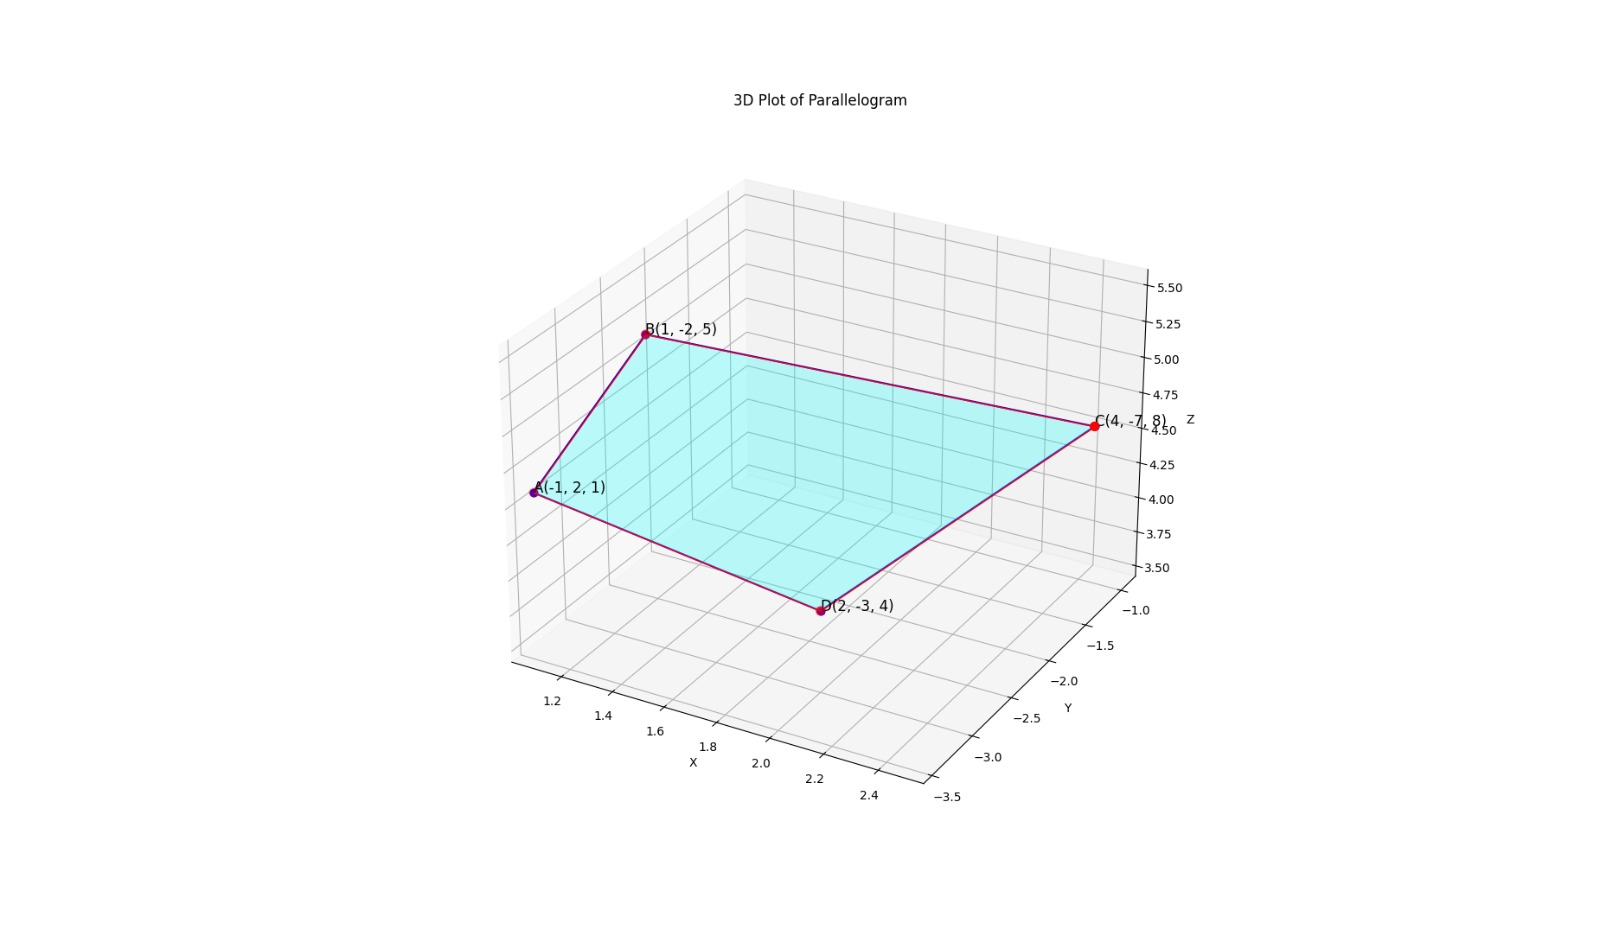
\includegraphics[width=0.7\linewidth]{IMG.jpg}
   \caption{Stem Plot of y\brak{n}}
     \label{stemplot}
\end{figure}

\numberwithin{equation}{enumi}
\numberwithin{figure}{enumi}
\renewcommand{\thetable}{\theenumi}



\end{document}  
